\documentclass[11pt]{article}

\usepackage[margin=1in]{geometry}
\usepackage{amsmath,amssymb}
\usepackage{hyperref}
\usepackage{graphicx}
\usepackage{enumitem}
\newcommand{\vect}[1]{\mathbf{#1}}
\newcommand{\mat}[1]{\mathbf{#1}}

\title{Reply Notes for Emilien Ouvrard}
\author{Sebastian Ares de Parga}
\date{May 13, 2026}

\begin{document}
\maketitle

\section*{Direct answers to your questions}

Your setup and your diagnostics are sensible. You are asking the right questions.

\subsection*{You wrote: ``I am not yet using Galerkin/LSPG, I am testing whether GPR can learn $k \mapsto q(k)$.''}

That is a good first test. And since you already state this clearly, I will only make the distinction explicit so we are fully aligned.

In your current test, you learn a direct map
\[
k \mapsto \vect{q}_N(k).
\]
with reconstruction
\[
e_h(k)\approx \mat{V}_N \vect{q}_N(k).
\]

In the closure setup, we split
\[
\mat{V}_N=[\mat{V}_p\;\mat{V}_s],\qquad
\vect{q}_N=
\begin{bmatrix}
\vect{q}_p\\
\vect{q}_s
\end{bmatrix},
\]
where \(\vect{q}_p\) are the retained/primary coefficients and \(\vect{q}_s\) are the secondary coefficients.

Then the learned relation is typically
\[
\vect{q}_s \approx g(\vect{q}_p),
\]
and \(\vect{q}_p\) comes from the reduced projection solve (Galerkin or LSPG), not from direct regression on \(k\). In intrusive form:
\[
\vect{q}_p(k)=\arg\min_{\vect{q}_p}\left\|R\!\left(\mat{V}_p \vect{q}_p+\mat{V}_s g(\vect{q}_p);k\right)\right\|^2.
\]
So yes, both approaches use GPR, but they are different regression problems. Because of that, if direct POD-GPR on \(k\mapsto \vect{q}_N\) struggles, it does \emph{not} automatically mean PROM-GPR will fail.

\subsection*{Your Question 1: ``Are you surprised by irregularity in modes 12--19? Should these be smoother?''}

I am not surprised.

I will refer to \(q_i\) as coefficients (not modes). Higher-index POD coefficients usually carry lower-energy and more oscillatory/localized content. They are often less regular and more sensitive to:
\begin{itemize}[leftmargin=1.5em]
    \item sampling density in parameter/frequency,
    \item numerical conditioning near resonances.
\end{itemize}

To be very direct: in my Burgers case, if I take one test trajectory and plot coefficients \(q_1\)--\(q_4\), \(q_{21}\)--\(q_{24}\), and \(q_{101}\)--\(q_{104}\), the first coefficients are clean and structured while higher-index coefficients are clearly rougher (see Figure A). Then, when I compare true vs predicted on the same trajectory (Figure B), the larger errors concentrate in the highest-index coefficients. So this roughness pattern is something we do see in practice; it is not, by itself, a red flag.

The two checks I would prioritize first are:
\begin{itemize}[leftmargin=1.5em]
    \item POD singular-value decay and cumulative energy: if those irregular coefficients belong to very low-energy directions, their impact on the reconstructed field is usually limited.
    \item Plot \(\Re(q_i)\) and \(\Im(q_i)\) directly, not only \(|q_i|\): for complex coefficients, the modulus can look artificially jagged when amplitude is small and phase rotates.
\end{itemize}

\subsection*{Your Question 2: ``What was the shape of your data? Is GPR still suitable?''}

This is a key point.

In our workflow, the effective training set is usually built \emph{per snapshot state}, not only per parameter point. So we often have many more training rows than ``number of parameter samples''.

For example, in one of our reference runs (different PDE, but same data-organization idea), we had:
\begin{itemize}[leftmargin=1.5em]
    \item \(\vect{q}_p \in \mathbb{R}^{20 \times 4509}\),
    \item \(\vect{q}_s \in \mathbb{R}^{131 \times 4509}\),
    \item test trajectories with 501 time samples.
\end{itemize}

So the model sees thousands of state samples, not only a few dozen parameter points.

In your current direct-frequency map, with around 90 training frequencies and one scalar input ($k$), GPR can still be a good choice, but it is a tougher regime for learning all coefficients at once.

\subsection*{Linear PROM performance: how I would interpret it}

Before deciding on nonlinear closure, I would still check a linear PROM baseline very carefully.

There are two practical cases:
\begin{itemize}[leftmargin=1.5em]
    \item If linear PROM is already accurate with relatively few retained coefficients, there may be no urgent need for PROM-GPR.
    \item If linear PROM needs many retained coefficients to reach the target accuracy, that is exactly the regime where PROM-GPR can be useful to reduce online dimension.
\end{itemize}

So if direct POD-GPR (\(k\mapsto \vect{q}_N\)) is weak, I would not stop there. I would still:
\begin{itemize}[leftmargin=1.5em]
    \item first secure accuracy with linear PROM (even if many coefficients are needed),
    \item then use PROM-GPR to compress/recover accuracy with a smaller effective online dimension.
\end{itemize}
In other words, there are problems where an intrusive, physics-based PROM is necessary because a purely non-intrusive map (for example direct POD-GPR or POD-DNN without projection/physics in the loop) is difficult to learn robustly.

\subsection*{Your Question 3: ``What method could handle rough data? DNN maybe?''}

With your current data volume, I would still start by pushing GPR further before moving to DNNs.

Concretely, I would test:
\begin{itemize}[leftmargin=1.5em]
    \item one GP per output coefficient (instead of one shared multi-output fit), so each coefficient can have its own kernel and its own shape/lengthscale parameters;
    \item kernel families beyond a single smooth stationary choice (for example Mat\'ern vs RBF vs Rational Quadratic, and combinations), because wave-like responses can require different regularity assumptions coefficient-by-coefficient;
    \item sparse/inducing-point GP variants if you later scale to much larger datasets (with 90 samples this is usually not required, but it can matter once your dataset grows).
\end{itemize}

For anisotropy/ARD: the key point is that ARD assigns one lengthscale per \emph{input feature}. If input is only \(k\), there is only one input-direction lengthscale. In a PROM-GPR closure setting, input becomes \(\vect{q}_p\), so input dimension is \(n_p\) and ARD becomes much more meaningful (one lengthscale per component of \(\vect{q}_p\)). You still can have different shape parameters across coefficients by fitting independent GP models per output coefficient.

About error interpretation: a relative error of around 15\% on a high-index coefficient does not necessarily imply a 15\% solution error. Two reasons:
\begin{itemize}[leftmargin=1.5em]
    \item high-index coefficients often have lower energy, so their contribution to the reconstructed field is smaller;
    \item for oscillatory/wave-like signals, relative coefficient error can be inflated by phase shift or local amplitude mismatch, even when the global field discrepancy is moderate.
\end{itemize}

So I would report both:
\begin{itemize}[leftmargin=1.5em]
    \item coefficient-level errors (relative and absolute),
    \item and solution-level metrics (field norm errors, plus phase/amplitude-aware metrics when relevant; Wasserstein-type metrics can also be informative in some settings).
\end{itemize}

\section*{Optional supporting figures}

\subsection*{A. Typical low-vs-high mode behavior}

\begin{figure}[h!]
    \centering
    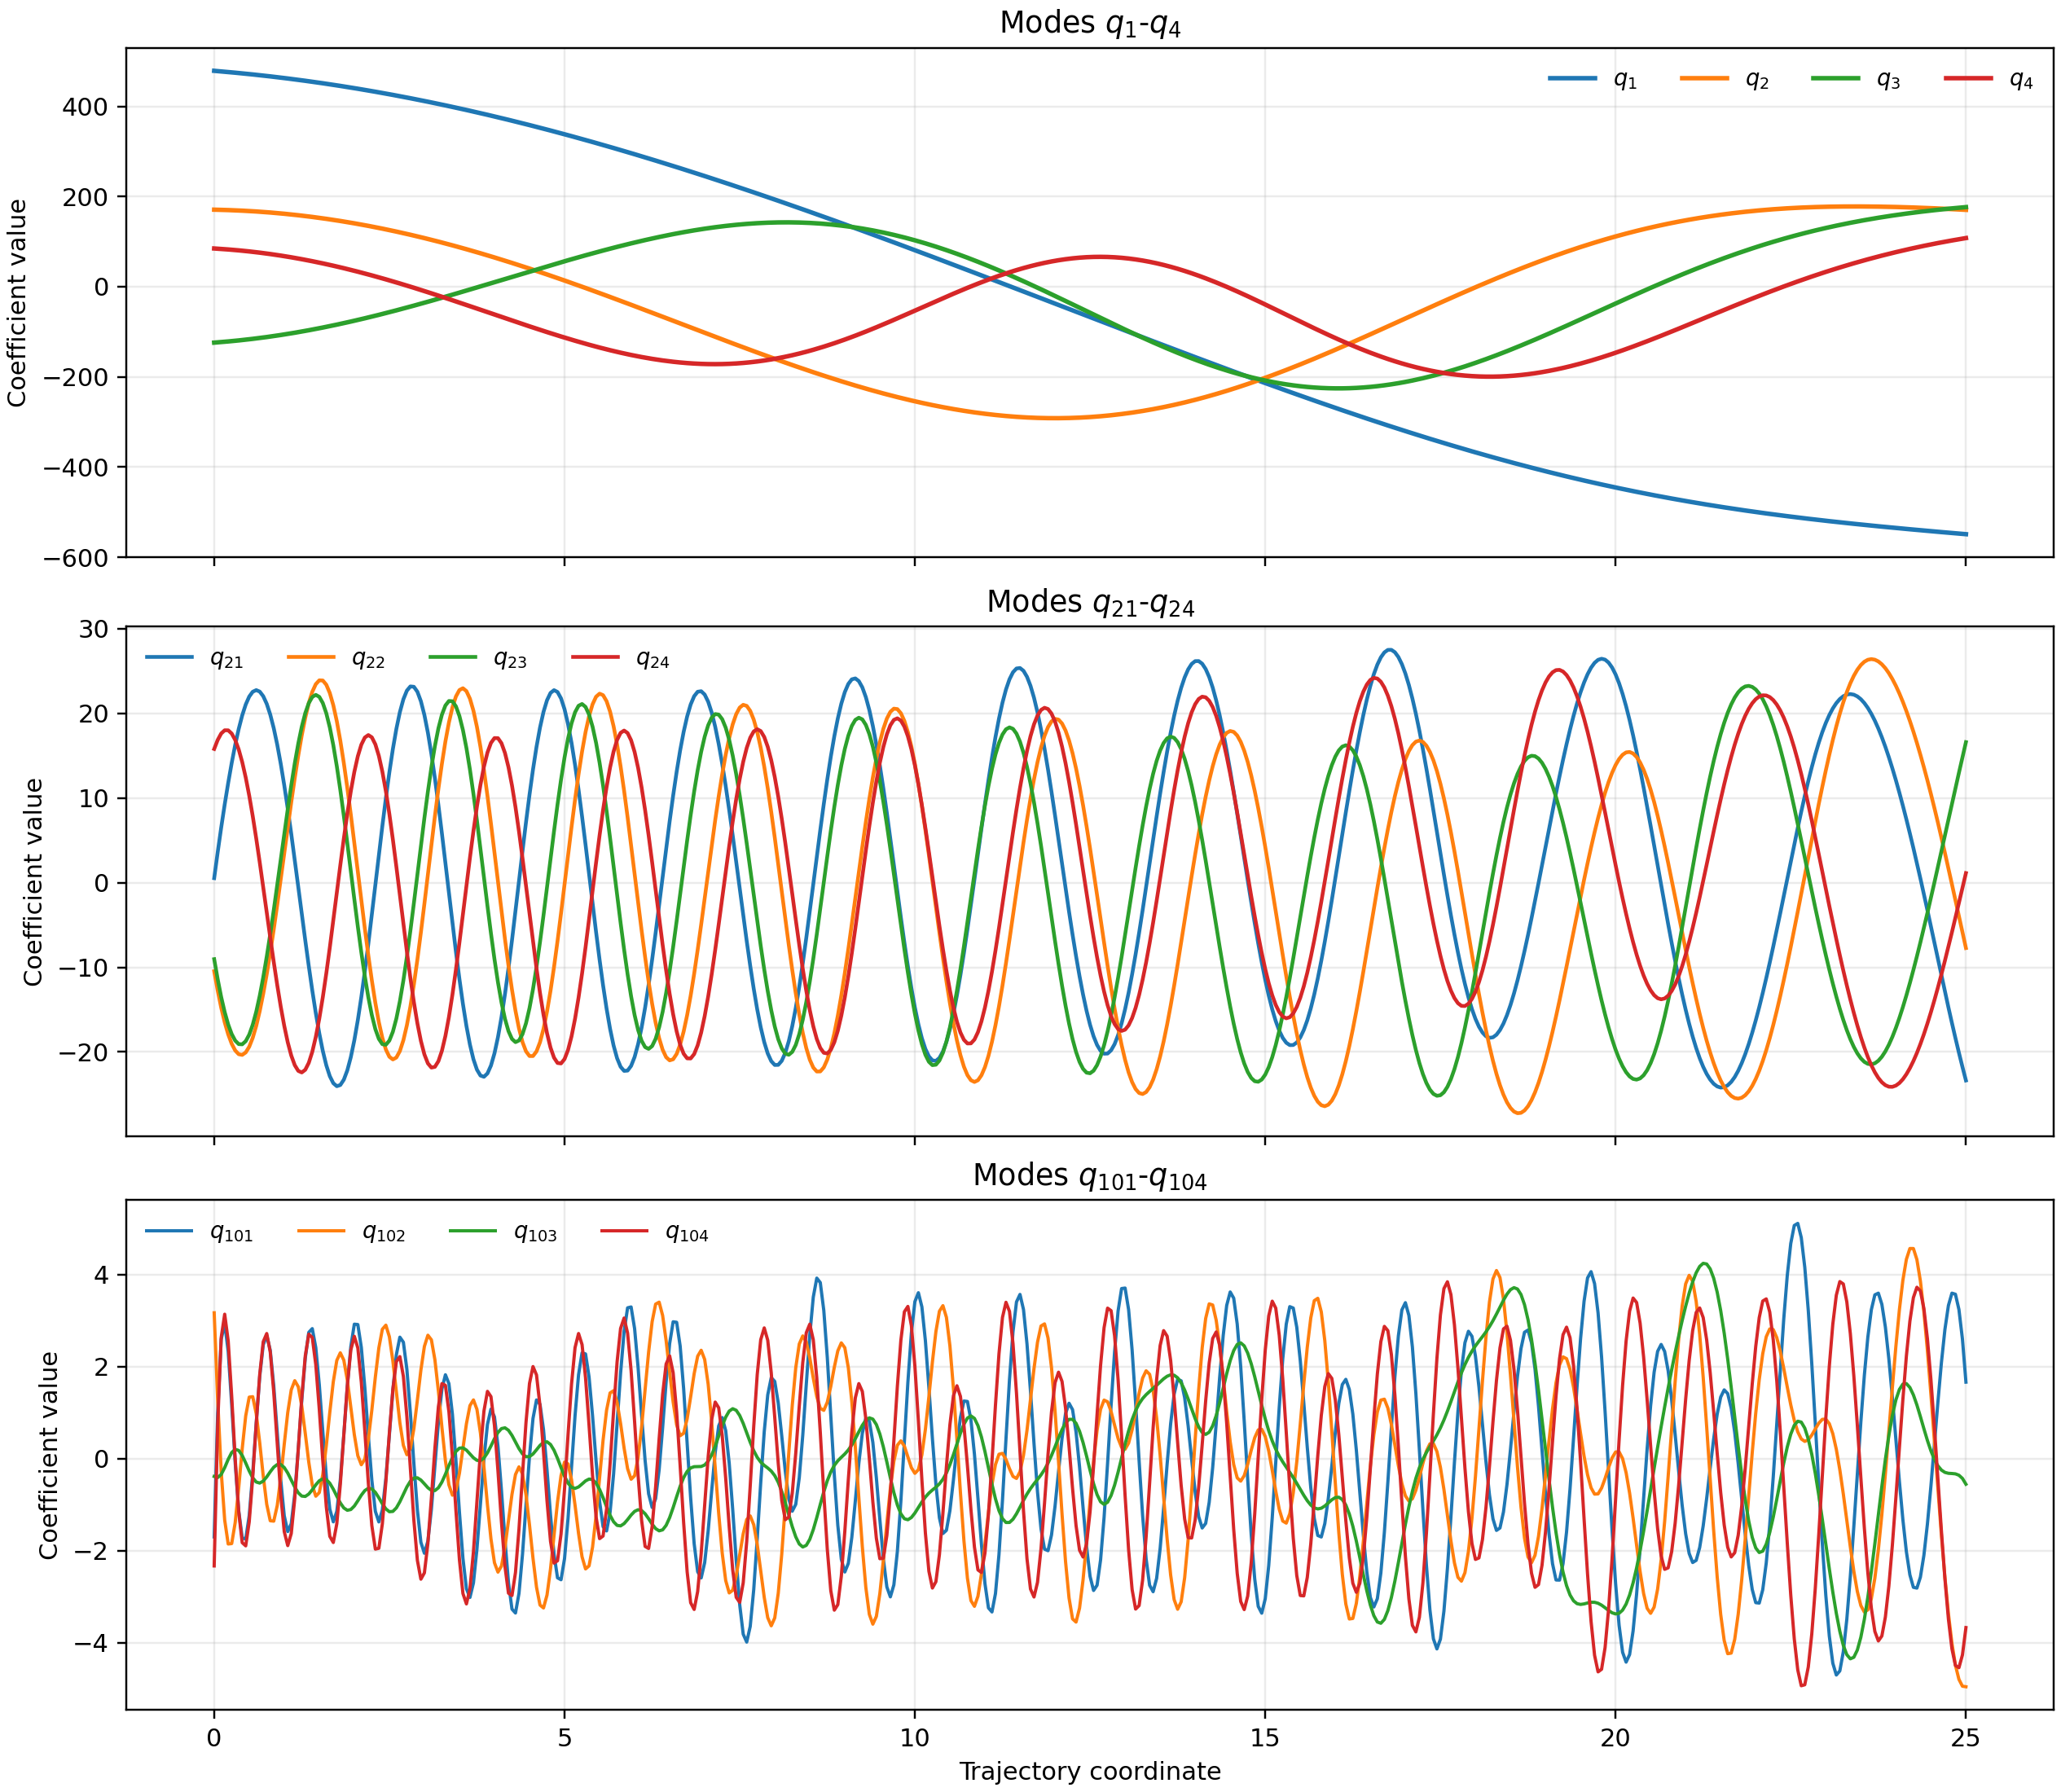
\includegraphics[width=0.95\textwidth]{figures/low_vs_high_modes_mu1_5.500_mu2_0.0150.png}
    \caption{Illustrative coefficient trajectories from one internal test trajectory using the three requested blocks: $q_1$--$q_4$, $q_{21}$--$q_{24}$, and $q_{101}$--$q_{104}$.}
\end{figure}

\subsection*{B. True vs predicted overlays at test point $(4.56, 0.019)$}

\begin{figure}[h!]
    \centering
    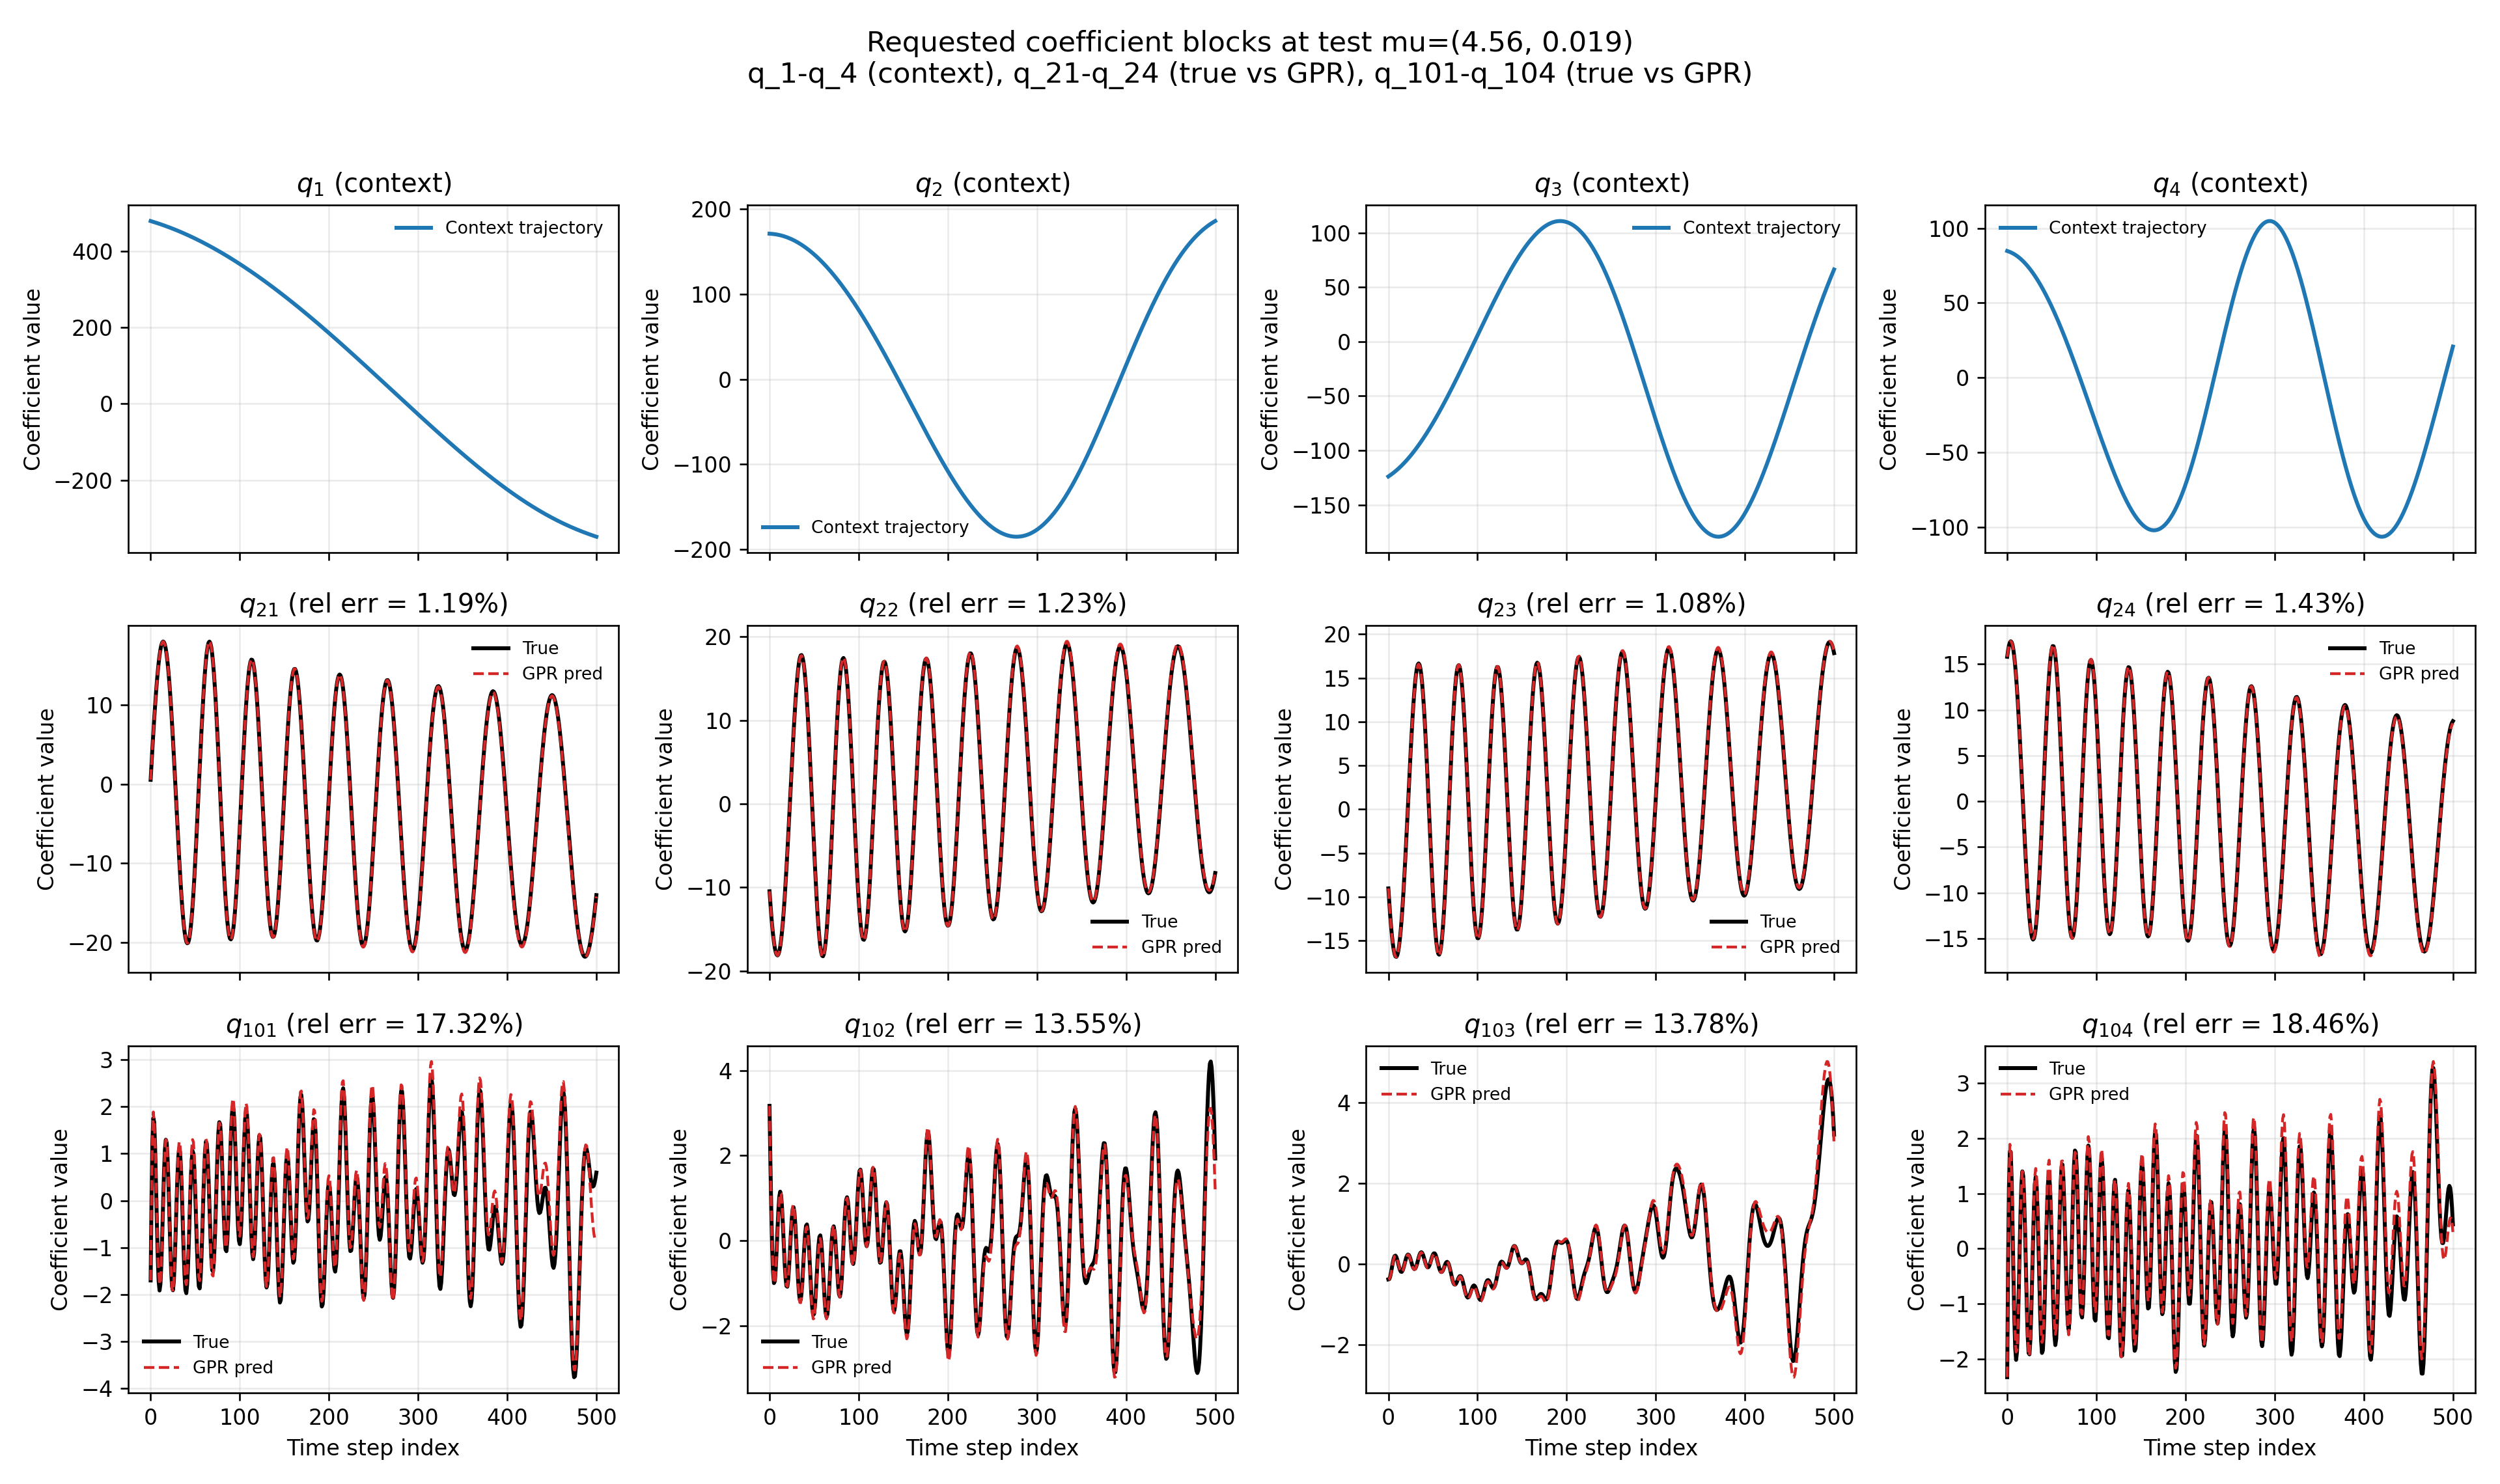
\includegraphics[width=0.98\textwidth]{figures/gpr_vs_true_modes_1_4_and_101_104_mu1_4.56_mu2_0.019.png}
    \caption{Coefficient overlays with the requested blocks: $q_1$--$q_4$, $q_{21}$--$q_{24}$, and $q_{101}$--$q_{104}$. Here $q_1$--$q_4$ are shown as context coefficients, while $q_{21}$--$q_{24}$ and $q_{101}$--$q_{104}$ are secondary coefficients with true-vs-GPR comparison.}
\end{figure}

\end{document}
